\documentclass{article}
\usepackage[utf8]{inputenc}
\usepackage{kotex}
\usepackage{url}
\usepackage{cancel}
\usepackage{xspace}
\usepackage{graphicx}
\usepackage{multicol}
\usepackage{multirow}
\usepackage{subfig}
\usepackage{amsmath}
\usepackage{amssymb}
\usepackage[a4paper, width=186mm, top=18mm, bottom=18mm, includeheadfoot]{geometry}
\usepackage{booktabs}
\usepackage{array}
\usepackage{verbatim}
\usepackage{caption}
\usepackage{natbib}
\usepackage{booktabs}   
\usepackage{float}
\usepackage{pdflscape}
\usepackage{mathtools}
\usepackage[usenames, dvipsnames]{xcolor}
\usepackage{afterpage}
\usepackage{pgf}
\usepackage{tikz}
\usepackage{dirtree}
\usepackage[style=american]{csquotes}
\usepackage{amsfonts}
\usepackage{tikz}
\usepackage{tkz-graph}
\usetikzlibrary{arrows,decorations.pathmorphing,automata,positioning,backgrounds,fit,shapes.symbols,chains,intersections}


\newtheorem{definition}{정의}[section]
\newtheorem{theorem}{Theorem}[section]
\newtheorem{lemma}{Lemma}
\newtheorem{proof}{Proof} [section]



\usepackage[toc, page, title, titletoc, header]{appendix}
\usepackage{marginnote}
\usepackage{tablefootnote}



%\renewcommand\appendixname{첨\부}
%\renewcommand\appendixpagename{첨\부}
%\renewcommand\appendixtocname{첨\부}
\renewcommand\abstractname{개요}


\usepackage{perpage} %the perpage package
\MakePerPage{footnote} %the perpage package command

\usetikzlibrary{shapes.geometric}%
\usepackage{color}
%\usepackage[pages=some, placement=top]{background}
\usepackage{eso-pic}
\usepackage[final]{pdfpages}

%\includepdf[pages=1]{cover}
\hyphenpenalty=750

\title{\textbf{Loopring(루프링):\\ 탈중앙화 토큰 거래 프로토콜}}

\author{	
	Daniel Wang\\	
	\texttt{daniel@loopring.org}\\	
	\and	
	Jay Zhou\\	
	\texttt{jay@loopring.org}\\	
	\and	
	Alex Wang\\	
	\texttt{alex@loopring.org}\\	
	\and	
	Matthew Finestone\\	
	\texttt{matt.finestone@gmail.com}\\	
	\\	
	\texttt{https://loopring.org}	
}


\makeatletter
\def\kotex@section@format{\Large\bfseries}
\makeatother

\makeatletter
\newenvironment{tablehere}
{\def\@captype{table}}
{}

\newenvironment{figurehere}
{\def\@captype{figure}}
{}
\makeatother

\begin{document}
\maketitle

\begin{abstract}
루프링은 탈중앙화 거래를 구축하기 위한 오픈 프로토콜이다. 루프링은 주문들을 종합하고 전달하는 오프 체인 그룹의 기능과 함께 거래 및 합의의 내용을 담은 공공의 스마트 계약들의 합으로 작동한다. 루프링 프로토콜은 무료이며, 확장 가능하고, 거래 기능을 포함하고 있는 분산형 응용 프로그램(dApps)을 위한 표준화된 구성 요소로 기능한다. 상호 운용이 가능한 기준은 인증을 필요로 하지 않는 익명 거래를 가능하게 한다. 현재 탈중앙화 거래 프로토콜에 대해 중요한 개선점은 주문을 다른 주문들과 조합(mix-and-match)하는 것을 통해, 두개의 거래 쌍으로만 거래가 가능하다는 제약을 없애고 주문서의 유동성을 향상할 수 있다는 것이다. 또한 루프링은 고유하고 솔루션을 사용하여 전면 운영(기존 거래보다 빠른 거래를 블록에 제출하려는 불공정한 시도)를 방지한다. 루프링은 특정 블록 체인에 구속 받지 않으며, 스마트 계약 기능을 갖춘 모든 블록 체인에 활용할 수 있다. 본 문서의 작성 시점에서, 이더리움(Ethereum)  \cite{buterin2017ethereum} \cite{wood2014ethereum} 및 큐텀(Qtum) \cite{dai2017smart}에서 작동이 가능하고 NEO \cite{atterlonn2018distributed} 설치가 진행 중입니다.
\end{abstract}



\begin{multicols}{2}
\linespread{1.5}
\section{도입\label{sec:introduction}}

블록체인 기반 자산의 급증으로 인해 거래처 간에 이들을 교환해야 할 필요성이 크게 증가했다. 전형적인 자산의 토큰화를 포함한 수천 개의 새로운 토큰이 도입됨에 따라 이러한 필요성은 더욱 확대되고 있다. 투기적 거래를 위한 동기부여를 위해서든, 그들의 고유 유틸리티 토큰을 통해 네트워크에 접속하기 위해 전환하든, 하나의 암호 장치를 다른 자산으로 교환하는 기능은 더 큰 생태계를 위한 토대가 된다. 자산 \cite{desotocapital}에는 잠재적 에너지가 있으며, 이 에너지 - 잠금 해제 된 자본- 를 실현하기 위해서는 블록 체인을 통해 소유권을 변경할 수 없게 하는 것뿐만 아니라, 이러한 자산을 자유롭게 양도하고 변환하는 기능이 필요하다. 

신원 보증을 필요로 하지 않는 토큰의 거래는 블록 체인 기술을 사용한 주목할 만한 사례이다. 하지만 현재까지 가상화폐의 열렬한 지지자들은 기존의 중앙 집중식 거래소를 통한 거래에 대체로 만족해 왔다. 비트코인 \cite{nakamoto2008bitcoin}이 P2P(사용자 간 직접 접속) 전자 화폐 거래와 관련해, “신뢰할 수 있는 제 3자가 이중 소비(double spending)를 막는 역할을 해야 한다면, 비트코인의 중요한 이점을 상실하게 되는 것이다”라고 지속적으로 강조하는 것과 같이, 탈 중앙화된 코인들이 반드시 신용할 수 있고 출입 제한이 있는 중앙 집중식 거래소를 통해야 한다면, 탈 중앙화된 자산들의 이점 역시 감소된다. 중앙 집중식 거래소에서 분산된 토큰을 거래하는 것은 냉정하게 보면 이치에 맞지 않다. 왜냐하면 이러한 분산된 프로젝트들이 옹호하는 탈중앙화와 거리가 있기 때문이다. 또한, 아래에 설명된 바와 같이 중앙 집중식 거래소를 통한 거래에는 수많은 실질적인 위험과 제한들이 있다. 탈 중앙화 거래소(DEX2) \cite{schuh2015bitshares} \cite{bancor} \cite{kyber}는 이러한 문제를 해결하기 위해 노력하고 있으며, 탈 금융 중개화를 위한 블록 체인을 사용함으로써 보안 위험을 완화시키는 데 성공해 왔다. 그러나 DEX의 기능이 발전해 새로운 경제체제에 있어 중요한 인프라가 되면서 성능 개선을 위한 실질적인 여지가 생겼다. 루프링은 여러 플랫폼에서 활용 될 수 있는 dApps 오픈 프로토콜을 사용해 해당 인프라에 모듈식 툴을 제공하는 것을 목표로 하고 있다.

	
	
\section{현재 거래소 환경\label{sec:current_exchange_landscape}}

\subsection{중앙 집중식 거래소의 부적절성}
중앙 집중식 거래소의 3가지 주요 위험 요소는 1)보안성 결여, 2)투명성 결여, 3)유동성 결여이다. 

\textbf{보안성 결여}는 전형적으로 사용자가 개인 소유의 키(펀드)에 대한 통제권을 하나의 중앙화된 독립체에 넘겨주면서 발생한다. 이는 사용자들의 중앙관리되는 자산들이 악의적인 해커의 먹잇감이 될 가능성에 노출시킨다. 모든 중앙 집중식 거래소에 발생하는 보안 및 해킹 위험은 잘 알려져 있지만 \cite{coincheckhack}  \cite{mcmillan2014inside} 이는 종종 토큰 거래를 위해 어쩔수 없이 용인되어야 할 "단점" 정도로 치부되기도 한다. 중앙 집중식 거래소의 서버는 사용자들의 수 백만 달러 이상의 자금을 관리하고 있기 때문에 많은 해커들의 공격 타겟이 되고 있다. 또한, 거래소의 개발자들은 이용자들의 자금으로 의도치 않은 우연한 오류를 발생시킬 수도 있다. 쉽게 말해, 사용자는 중앙 집중식  거래소에 그들의 토큰을 예치할 경우 이것을 직접 관리하지 못하는 것이다.

\textbf{투명성 결여}는 사용자들을 불공정한 행위로 인해 발생하는 부정한 거래의 위험에 노출시킨다. 여기서 부정함은 교환원의 악의적인 의도에 의해서 생긴다. 왜냐하면 사용자들이 그들의 자산을 중앙 집중식 거래소에 실제로 보관하는 것이 아니라, 전산상으로만 권리(IOU)를 거래하고 있기 때문이다. 거래소의 월렛에 코인을 보내면 거래소는 사용자의 계정에 해당하는 월렛에 보관하는 것이 아니라, 따로 보관하고 대신 계정에 이에 해당하는 권리(IOU)를 준다. 권리(IOU)의 이동을 통해 사용자의 계정들 사이의 모든 거래는 전송수수료 없이 효과적으로 이루어진다. 사용자들은 인출을 위해 그들이 가진 권리(IOU)를 거래소와 교환하고 코인을 다시 그들 외부의 월렛 주소로 받는다. 이와 같은 프로세스가 진행되는 내내 투명성이 결여되어 있기 때문에, 거래소가 폐쇄되거나 계좌 동결 및 파산 등의 상황이 발생할 수 있다. 또한 거래소가 보관 중인 사용자들의 자산을 제 3자에게 대출해 주는 등의 다른 목적으로 사용하는 것도 가능하다. 투명성의 결여는 더 높은 거래 수수료, 피크 수요의 지연, 규제 위험 및 전면 실행 명령과 등과 같은 자산의 전체 분실 없이도 사용자들에게 큰 대가를 치르게 할 수 있다.

\textbf{유동성의 결여}. 거래소를 교환원의 관점에서 볼 때, 분산된 유동성은 두개의 ‘승자독식’ 시나리오 때문에 새로운 거래소의 진입을 제한한다. 첫째, 사용자들은 자신들이 모든 거래를 한 거래소에서 수행하는 것이 유리하다고 생각하기 때문에 거래가능한 자산의 종류가 가장 많은 거래소가 이기게 된다. 둘째, 많은 매도, 매수 잔량을 가진 곳이 매수가와 매도가의 차이가 적어 유리하다. 이는 신규 업체들이 초기 유동성을 확보하기 어렵기 때문에 경쟁을 저해한다. 이러한 이유들로 인해, 사용자들의 온갖 불만과 대규모 해킹 사고에도 불구하고 큰 거래소들이 높은 시장 점유율 차지하고 있다. 중앙 집중식 거래소가 더 많은 시장 점유율을 차지할수록, 공격대상이 될 위험성은 점점 더 높아진다.

사용자 관점에서 분산된 유동성은 사용자 경험을 크게 감소시킨다. 중앙 집중식 거래소에서 사용자들은 그들이 이용하는 거래소의 주문서에 반영되어 있는 거래소 자체의 유동성 풀, 그리고 거래소에서 지원하는 자산으로만 거래를 할 수 있다. 코인 A를 코인 B로 교환하기 위해서 사용자는 개인 정보를 밝히고 A, B 두 코인을 지원하는 거래소로 가거나 서로 다른 거래소에 가야 한다. 사용자는 종종 전형적인 BTC또는 ETH를 통한 예비 혹은 중개 거래를 실행할 필요가 있고, 이 과정에서 스프레드에 따른 매매가격차액을 지불해야한다. 마지막으로, 주문서의 잔량은 가격의 변동 없이 거래를 완료하기에 충분치 않을 수 있다. 거래소가 대량으로 처리되도록 압력을 넣어도, 이 거래량과 유동성이 가짜가 아니라고 보장할 수는  없다 \cite{fakevolume}.

그 결과 기존의 금융 체계와 유사한 분산된 유동성 풀과 같은 분산 생태계가 형성되며, 대부분의 거래량이 몇몇 소수의 거래소에 집중된다. 중앙 집중식 거래소로 인해 블록 체인은 전세계의 유동성을 공언할 수 없게 되는 것이다.

\subsection{탈중앙화 거래소의 부적절성}
탈중앙화 거래소는 중앙 집중식 거래소와 부분적으로 다르다. 그 이유는 사용자들이 기본적으로 블록 체인 위에서 직접 거래함으로써 그들의 개인키 (자산)를 관리하기 때문이다. 암호 화폐 자체의 신용보증을 필요로 하지 않는 기술을 활용함으로써 그들은 보안과 관련하여 위에 언급된 위험의 대부분을 성공적으로 완화한다. 하지만 성능 및 구조상의 제약과 관련된 문제는 여전히 남아있다. 

유동성은 사용자들이 거래소마다 다른 유동성 풀과 거래를 원하는 자산들로 인해 종종 문제가 된다. 만일 DEXs 혹은 dApps 전반에 걸쳐 각각의 운영을 위해 일관된 기준을 적용하지 않고, 주문이 광범위한 네트워크에 걸쳐 공유/전파되지 않는다면, 분산된 유동성으로 인한 문제는 지속될 것이다. 지정가 주문서의 유동성, 특히 이들의 회복력 -지정가 주문이 얼마나 빨리 재생되는지- 은 최적 거래 전략에 상당한 영향을 미칠 수 있다 \cite{limitorderliquidity}. 이러한 기준의 부재는 유동성이 감소할 뿐만 아니라 잠재적으로 불안정한 스마트 계약들을 만들어 내고 있다.

뿐만 아니라, 거래가 체인에서 성사되기 때문에 DEXs는 기본적인 블록 체인의 태생적인 한계인 확장성, 실행(채굴) 지연 및 주문과정에서 비싼 수수료 등의 특징을 갖게 된다. 따라서, 블록 체인 주문서는 블록 체인에서 코드를 실행하는데 비용(gas)이 발생하기 때문에 확장이 잘 되지 않으며, 다수의 주문을 취소하는데 많은 비용이 들게 한다. 마지막으로, 블록 체인 주문서는 공공의 분야이므로, 다음 블록에 채굴되어 주문서에 기입되기를 기다리면서 채굴자에 의해 주문을 넣는 매매 내용은 공개적이게 된다. 이 같은 지연으로 인해 사용자는 거래 내용이 공개되고 공개된 가격을 활용해 다른 거래자들이 그들에게 유리하도록 호가를 변경하는 위험에 노출된다.

\subsection{하이브리드 솔루션} 
위와 같은 이유로, 순수하게 블록 체인 기반의 거래소는 중앙 집중식 거래소들에 비해 경쟁력이 낮아지는 문제를 가진다. 온 체인 고유의 탈중앙화와 중앙 집중식 거래소의 속도 및 명령 유연성 사이에는 균형점이 있다. 루프링 및 0x \cite{warren20170x}와 같은 프로토콜은 오프 체인에서의 주문 관리를 통해 온 체인 결제의 솔루션을 확장한다. 이 솔루션은 개방형 스마트 계약을 중심으로 돌아가지만, 네트워크에서 중요한 역할을 수행하기 위해 노드 유연성을 제공하고 몇 가지 오프 체인의 기능들을 수행함으로써 확장성 한계를 해결한다. 그러나, 하이브리드 모델에도 여전히 단점은 있다 \cite{costofdecent}. 루프링 프로토콜은 이 문서 전반에 걸쳐 하이브리드 솔루션에 대한 우리의 접근 방식의 의미 있는 차이점들을 설명할 것이다.



\section{루프링 프로토콜\label{sec:loopring_protocol}}
루프링은 DEX가 아니라 다수의 블록 체인에 DEX들을 구축하기 위한 모듈식 프로토콜이다. 우리는 기존 거래소의 구성 요소를 분해하고 그 대신에 일련의 공공 스마트 계약들과 분산된 행위자들을 제공한다. 
네크워크에서의 역할에는 월렛, 릴레이, 유동성 공유 컨소시엄 블록 체인, 주문서 브라우저, 링 채굴자, 자산 토큰화 서비스 등이 포함된다. 이들을 각각 정의하기 전에 우리는 먼저 루프링 주문을 이해해야 한다.

\subsection{주문 링\label{sec:order_ring}}
주문링은 우리가 흔히 단향성 주문 모델 (UDOM)이라고 부르는 방식으로 표현한다 \cite{coinport2014udom}. UDOM는 입찰 및 요청 대신에 토큰 교환 요청, amountS/amountB(매도/매입수량)으로 주문을 표현한다. 모든 주문은 두 토큰 사이의 환율이므로 루프링 프로토콜의 강력한 점은 다수의 주문을 원형 거래로 조합(mix-and-match)하는 것이다. 단일 거래 페어(쌍) 대신 최대 16개까지 주문을 활용함으로써, 유동성 및 가격 개선 가능성이 급격히 높아진다. 

\begin{center}
	\begin{figurehere}
		\centering
		\tikzstyle{block} = [draw, fill=blue!20, rectangle, 
		minimum height=3em, minimum width=6em]
		\tikzstyle{sum} = [draw, fill=blue!20, circle, node distance=1cm]
		\tikzstyle{input} = [coordinate]
		\tikzstyle{output} = [coordinate]
		\tikzstyle{pinstyle} = [pin edge={to-,thin,black}]
		
		\begin{tikzpicture}[
		auto, 
		node distance=2cm,
		>=latex',
		font=\bfseries\footnotesize\sffamily,
		order/.style={
			scale=0.7,
			rectangle,
			rounded corners,
			draw=black, 
			text centered,
			%		text width=5cm,
			minimum height=12mm,
			fill=white
		},
		label/.style={
			scale=0.7
		}
		]
		% We start by placing the blocks
		
		\node [order] (order2) 
		{%
			\begin{tabular}{l}
			\textbf{주문\#2}\\
			\textbf{소유주: Y}\\
			\textbf{매도수량: 9B}\\
			\textbf{매입수량: 12C}
			\end{tabular}
		};
		
		\node [order, below of=order2, xshift=-3.5cm] (order1) 
		{%
			\begin{tabular}{l}
			\textbf{주문\#1}\\
			\textbf{소유주: X}\\
			\textbf{매도수량: 10000A}\\
			\textbf{매입수량: 2B}
			\end{tabular}
		};
		
		
		\node [order, below of=order2, xshift=3.5cm] (order3) 
	{%
			\begin{tabular}{l}
			\textbf{주문\#3}\\
			\textbf{소유주: Z}\\
			\textbf{매도수량: 100C}\\
			\textbf{매입수량: 160A}
			\end{tabular}
		};
		
		\draw [draw,->] (order1) -- node [label] {\textbf{7898A}} (order3);
		\draw [draw,->] (order2) -| node [label, xshift=-1.8cm] {\textbf{8B}} (order1);
		\draw [draw,->] (order3) |- node [label, xshift=1cm, yshift=0.24cm] {\textbf{98C}} (order2);
		
		\end{tikzpicture}
		
\caption{3가지 주문의 주문 링}
		\label{fig:ring}
	\end{figurehere}

\end{center}

위의 그림은 3가지 주문의 주문 링을 보여준다. 각 주문의 판매를 위한 토큰(\verb|tokenS|)은 또 다른 주문의 구매를 위한 토큰(\verb|tokenB|)이다. 이것은 각 주문이 그것의 페어를 위한 서로 다른 주문을 통하지 않고 원하는 토큰을 직접 거래할 수 있도록 하는 루프를 생성한다. 물론 기존의 주문 거래는 주문 링의 특수한 경우에도 여전히 실행될 수 있다.

\begin{definition}[주문 링] $C_{0}$, $C_{1}$, $\cdots$, $C_{n-1}$은 $n$개의 서로 다른 토큰으로 하고, $O_{0\rightarrow 1}$, $\cdots$, $O_{i\rightarrow i\oplus 1}$, $\cdots$, $O_{n-1 \rightarrow 0}$은 $n$개의 주문으로 한다. 이러한 주문들은 거래를 위한 주문 링을 형성한다:

$$O_{0\rightarrow 1} \rightarrow \cdots \rightarrow O_{i\rightarrow i\oplus 1} \rightarrow \cdots \rightarrow O_{n-1\rightarrow 0} \text{, }$$

$n$이 주문 링의 길이, 그리고 $i\oplus 1 \equiv i+1 \mod n$.

\end{definition}

주문 링은 모든 구성 요소 거래들이 사용자들에게 암시적으로 지정된 기존 환율보다 낫거나 동일한 환율로 진행될 수 있는 거래일 때 유효한 것으로 본다. 주문 링의 유효성을 검증하기 위해, 루프링 프로토콜의 스마트 계약은 반드시 모든 주문의 원래 환율의 결과가 1이상일 때 링 채굴자로부터 주문 링을 받아야 한다.

앨리스와 밥이 그들의 토큰  \verb|A| 와 \verb|B| 거래하고 싶어한다고 가정해보자. 앨리스는 갖고 있는 15개의 토큰  \verb|A|를 4개의 토큰\verb|B|로 거래하길 한다. 그리고 밥은 10개의 토큰 \verb|B|를 가지고 있고 그것으로 30개의 토큰 \verb|A|를 원한다.

누가 판매를 하고 누가 구매를 하고 있을까? 이는 오직 가격견적을 하기위해 우리가 정한 자산에 따른다. 만약 토큰 \verb|A|가 참조일 때, 엘리스는 토큰 \verb|B|를 $\frac{15}{4}$ = 3.75\verb|A|의 가격에 구매하는 것이고, 밥은 10개의 토큰 \verb|B|를 $\frac{30}{10}$ = 3.00\verb|A|의 가격에 판매하는 것이다. 토큰 \verb|B|를 참조로 정할 경우, 엘리스는 15개의 토큰 \verb|A|를 $\frac{4}{15}$ = 0.26666667\verb|B|의 가격에 판매하는 것이고, 밥은 10개의 토큰 \verb|A|를 $\frac{10}{30}$ = 0.33333334\verb|B|의 가격에 구매하는 것이다. 따라서, 누가 구매자이고 판매자인지는 임의적이다. 
첫번째 상황에서 앨리스는 밥이 팔려고 하는 가격(3.00\verb|A|)보다 더 높은 가격(3.75 \verb|A|)을 지불하려고 하는 반면, 두번째 상황에서는 밥이 엘리스가 팔려고 하는 가격(0.26666667\verb|B|)보다 더 높은 가격(0.33333334\verb|B|)을 지불하려고 한다. 구매자가 판매자의 가격과 같거나 더 높은 가격을 지불하려고 할 때는 거래가 가능하다는 것은 명백하다.

\begin{equation}
{{15\over 4} \over {30\over 10}} = {{10\over 30} \over {4\over 15}}={15 \over 4} \cdot {10 \over 30} = 1.25 > 1
\end{equation}

그러므로 N개의 주문 집합이 전체 또는 부분적으로 성사될 수 있도록 하기 위해, 우리는 구매 주문서에 있는 각 환율의 결과가 1보다 크거나 동일한 수가 있는 지 알아야 한다. 만일 그렇다면, 모든 N개의 주문이 부분적으로 또는 완전히 성사될 수 있다 \cite{supersymmetry}.
세번째 당사자인 찰리가 있다. 앨리스가 x1의 토큰 \verb|A|를 주고 y1의 토큰 \verb|B|를 받고 싶어하고 밥은 x2의 토큰 \verb|B|를 주고 y2의 토큰 \verb|C|를 받고 싶어한다. 그리고 찰리는 x3의 토큰 \verb|C|를 주고 y3의 토큰 \verb|A|를 받고 싶어 한다. 필요한 토큰은 존재하며, 다음과 같을 경우 거래는 가능하다:

\begin{equation}
	{{x_1 \cdot x_2 \cdot x_3 \over y_1 \cdot y_2 \cdot y_3}\geq 1}
\end{equation}

루프링 주문에 관한 더 자세한 사항은 제 7.1항을 참고한다.  



\section{생태계 참여자들\label{sec:ecosystem}}
다음의 생태계 참여자들은 중앙 집중식 거래소가 제공해야 하는 모든 기능을 공동으로 제공하고 있다.

\begin{itemize}
	
	\item \textbf{월렛:} 사용자에게 토큰에 대한 접근 권한과 루프링 네트워크에 주문을 보내는 방법을 제공하는 일반적인 월렛 서비스 또는 인터페이스다. 월렛은 링 채굴자와 수수료를 공유함으로써 주문을 생산하는데 인센티브를 받게 될 것이다 (제 8항 참조). 향후의 거래가 각 사용자의 월렛을 통해 안전하게 이뤄질 것이라는 믿음과 함께, 우리의 프로토콜을 통해 월렛의 유동성 풀을 연결하는 것은 큰 중요성을 갖는다.

	\item \textbf{유동성 공유 블록 체인/릴레이-메시 컨소시엄:} 주문 및 유동성 공유를 위한 릴레이-메시 네트워크. 노드가 루프링 릴레이 소프트웨어를 실행할 때, 그들은 기존 네트워크에 합류할 수 있고 컨소시엄 블록 체인 위에 다른 릴레이들과 유동성을 공유할 수 있다. 우리가 최초의 이행으로 구축할 컨소시엄 블록 체인은 거의 실시간으로 주문을 공유(1-2초 블록) 하며, 새로운 노드를 활용해 이전 기록을 더 빨리 다운로드하는 것을 가능케 한다. 주목할만한 것은, 릴레이는 이 컨소시엄에 합류할 필요가 없다는 것이다. 릴레이는 단독으로 작용하여 다른 것들과 유동성을 공유하지 않을 수 있으며 자체의 유동성 공유 네트워크를 생성 및 관리할 수 있다.

	\item \textbf{릴레이/링 채굴자들:} 릴레이는 월렛 또는 릴레이 메시로부터 주문을 받고, 공공 주문서 및 거래 내역을 유지 관리하며 선택적으로 주문을 다른 릴레이(임의의 오프체인 매체를 통해) 그리고/또는 릴레이 메시 노드에게 알리는 노드이다. 링 채굴은 릴레이의 – 요구 사항이 아닌 - 특징이다. 이는 많은 계산이 요구되고, 완전하게 오프 체인으로 되어 있다. 링 채굴의 특징이 있는 릴레이를 “링-채굴자”라고 부르는데, 이 릴레이는 서로 다른 주문들을 함께 이어서 주문 링을 생성한다. 릴레이는 (1) 다른 릴레이와 의사 소통하는 방법, (2) 주문서 작성 방법, 그리고 (3) 어떻게 주문 링(채굴 알고리즘)을 채굴하는지에 있어 자유롭다.

	\item \textbf{루프링 프로토콜 스마트 계약 (LPSC):} 링 채굴자로부터 받은 주문 링을 체크하고 사용자들을 대신해 신용 없이 토큰을 합의하고 전송하는 인련의 공공 및 자유 스마트 계약은 링 채굴자와 수수료가 있는 월렛에 인센티브를 주고 이벤트를 내보낸다. 릴레이/주문 브라우저는 그들의 주문서와 거래 기록을 최신 버전으로 유지하기 위해 이같은 이벤트에 주목한다. 자세한 내용은 부록을 참조한다.

	\item \textbf{자산 토큰화 서비스 (ATS):} 루프링에서 직접 거래될 수 없는 자산들을 연결하는 역할. 신뢰할 수 있는 기업이나 조직에 의해 운영되는 중앙 집중식 서비스들이다. 사용자들은 자산(실제, 지시 또는 다른 체인에서의 토큰)을 예치하고 발행된 토큰을 얻는데, 이는 나중에 예치금으로 다시 바꿀 수 있다. 루프링은 크로스 체인 거래 프로토콜이 아니라 (적당한 솔루션이 마련될 때까지) 다른 블록 체인의 자산 뿐만아니라 물질적 자산을 갖춘 ERC20 토큰 \cite{ERC20}의 거래를 가능하게 하는 ATS다.

\end{itemize}



\section{거래 과정\label{sec:process}}

\begin{enumerate} 
	
	\item \textbf{프로토콜 승인}: figure 2에서, 토큰 거래를 원하는 사용자 \verb|Y|는 \verb|LPSC|를 사용자가 판매를 원하는 토큰 \verb|B|의 매도수량(\verb|amountS|)를 처리할 수 있도록 승인한다. 이는 주문이 진행되는 동안 여전히 토큰을 자유롭게 이동시킬 수 있는 사용자가 소유한 토큰의 움직임에 제약을 두지 않는다.
	
	\item \textbf{주문 생성}: 토큰 \verb|C| 대 토큰 \verb|B|에 대한 현재 비율 및 주문서는 주문서 브라우저와 같이 네트워크에 연결된 릴레이 또는 기타 에이전트에 의해 제공된다. 사용자 \verb|Y|는 모든 통합된 월렛 인터페이스를 통해 원하는 매도수량(\verb|amountS|), 원하는 매입수량(\verb|amountB|) 및 기타 매개 변수를 지정하는 주문(지정가 주문)을 한다. 링 채굴 비용으로 주문에 LRx의 일정액이 추가될 수 있다; LRx의 비용이 더 높다는 것은 링 채굴자에 의해 더 일찍 처리되기 위한 더 나은 기회를 의미한다. 주문 해시는 사용자 \verb|Y|의 개인 키로 서명된다.
	
    \item \textbf{주문 브로드캐스트}: 월렛은 하나 혹은 그 이상의 릴레이에 주문 및 서명을 전달한다. 릴레이는 그것의 공공 주문서를 업데이트한다. 이 프로토콜은 주문서가 선착순과 같은 특정 방식으로 작성될 것을 요구하지 않는다. 대신에, 릴레이는 주문서를 만들 때 자체 설계 결정을 내릴 수 있는 권한을 가지고 있다. 
    
    \item \textbf{유동성 공유}: 릴레이는 임의의 통신 매체를 통해 주문을 다른 릴레이로 브로드캐스트한다. 다시 한번, 노드들이 어떤식으로 상호 작용하는지/상호 작용할 것인지 말 것인지에 대한 유연성은 있다. 특정 수준의 네트워크 연결을 용이하게 하기 위해, 컨소시엄 블록 체인을 이용한 유동성 공유 릴레이 메시가 내장되어 있다. 앞서 언급했듯이, 이러한 릴레이 메시는 속도와 포괄성에 최적화되어 있다.

\begin{center}
	\begin{figurehere}
		\centering
		\tikzstyle{block} = [draw, fill=blue!20, rectangle, 
		minimum height=3em, minimum width=6em]
		\tikzstyle{sum} = [draw, fill=blue!20, circle, node distance=1cm]
		\tikzstyle{input} = [coordinate]
		\tikzstyle{output} = [coordinate]
		\tikzstyle{pinstyle} = [pin edge={to-,thin,black}]
		
		\begin{tikzpicture}[
		auto, 
		scale=0.7,
		node distance=2cm,
		>=latex',
		font=\bfseries\footnotesize\sffamily,
		order/.style={
			rectangle,
			scale=0.7,
			rounded corners,
			draw=black, 
			text centered,
			%		text width=5cm,
			minimum height=12mm,
			minimum width=30mm,
			fill=white
		},
		role/.style={
			circle,
			scale=0.7,
			draw=black, 
			text centered,
			%		text width=5cm,
			minimum height=12mm,
			minimum width=12mm,
			fill=white
		},
		steps/.style={
			circle,
			scale=0.7,
			draw=black, 
			text centered,
			%		text width=5cm,
			%		minimum height=12mm,
			%		minimum width=12mm,
			fill=black,
			text=white
		},
		account/.style={
			circle,
			scale=0.7,
			draw=black, 
			text centered,
			%		text width=5cm,
			minimum height=16mm,
			minimum width=16mm,
			fill=white
		},
		label/.style={
			scale=0.7
		}
		]
		
		
		\node [role] (user1)  {사용주 X};
		\node [role, below of=user1] (user2)  {사용자 Y};
		\node [role, below of=user2] (user3)  {사용자 Z};
		\node [role, below of=user3, fill=gray!20] (relay1)  {릴레이 M};
		\node [role, below of=relay1, fill=gray!20] (relay2)  {릴레이 N};
		
		
		\node [order, left of=user1, xshift=-1cm] (order1) 
		{%
			\begin{tabular}{l}
			\textbf{주문 1}\\
			\textbf{소유주: X}\\
			\textbf{매도수량: 10000 A}\\
			\textbf{매입수량: 2 B}
			\end{tabular}
		};
		
		\draw [draw, ->]  (user1) -- (order1) [label]{};
		\draw [bend right,->] (order1) to node [auto, scale=0.7] {} (relay1);
		\draw [bend right,->] (order1) to node [auto, scale=0.7] {} (relay2);
		% \draw [draw, ->]  (order1) |- (relay1) [label]{};
		% \draw [draw, ->]  (order1) |- (relay2) [label]{};
		
		\node [order,left of=user2, xshift=-1.5cm] (order2) 
		{%
			\begin{tabular}{l}
			\textbf{주문 2}\\
			\textbf{소유주: Y}\\
			\textbf{매도수량: 9  B}\\
			\textbf{매입수량: 12 C}
			\end{tabular}
		};
		\draw [draw, ->]  (user2) -- (order2) [label]{};
		\draw [bend right,->] (order2) to node [auto, scale=0.7] {} (relay1);
		\draw [bend right,->] (order2) to node [auto, scale=0.7] {} (relay2);
		% \draw [draw, ->]  (order2) |- (relay1) [label]{};
		% \draw [draw, ->]  (order2) |- (relay2) [label]{};
		% 
		\node [order, left of=user3, xshift=-2cm] (order3) 
		{%
			\begin{tabular}{l}
			\textbf{주문 3}\\
			\textbf{소유주: Z}\\
			\textbf{매도수량: 100 C}\\
			\textbf{매입수량: 160 A}
			\end{tabular}
		};
		\draw [draw, ->]  (user3) -- (order3) [label]{};
		\draw [bend right,->] (order3) to node [auto, scale=0.7] {} (relay1);
		\draw [bend right,->] (order3) to node [auto, scale=0.7] {} (relay2);
		% \draw [draw, ->]  (order3) |- (relay1) [label]{};
		% \draw [draw, ->]  (order3) |- (relay2) [label]{};
		
		% // The Ring
		\node [order, 
		yshift=-1.5cm,
		xshift=-2.75cm,
		below of=relay2,
		fill=gray!10,
		minimum width=4.2cm,
		minimum height=5cm] (ring) {};
		
		
		\node [order, dashed, below of=relay2,yshift=-0.2cm,xshift=-2.5cm] (order11) 
		{%
			\begin{tabular}{l}
			\textbf{주문 1}\\
			\textbf{소유주: X}\\
			\textbf{매도수량: 10000 A}\\
			\textbf{매입수량: 2 B}
			\end{tabular}
		};
		\node [order, dashed,below of=order11,xshift=-0.25cm,yshift=0.7cm] (order21) 
		{%
			\begin{tabular}{l}
			\textbf{주문 2}\\
			\textbf{소유주: Y}\\
			\textbf{매도수량: 9  B}\\
			\textbf{매입수량: 12 C}
			\end{tabular}
		};
		\node [order, dashed,below of=order21,xshift=-0.25cm,yshift=0.7cm] (order31) 
		{%
			\begin{tabular}{l}
			\textbf{주문 3}\\
			\textbf{소유주: Z}\\
			\textbf{매도수량: 100 C}\\
			\textbf{매입수량: 160 A}
			\end{tabular}
		};
		
		% // The blockchain
		\node [
		rectangle,
		fill=gray!20, 
		right of=user1,
		yshift=-4.5cm,
		xshift=0.1cm,
		scale=0.7,
		minimum width=3.2cm,
		minimum height=15.6cm] (blockchain) {\parbox[b][15cm]{1.3cm}{블록체인}};
		% blockchain accounts
		\node [account, right of=user1, xshift=1cm] (account1)  {계정X};
		\node [account, right of=user2, xshift=1cm] (account2)  {계정Y};
		\node [account, right of=user3, xshift=1cm] (account3)  {계정Z};
		\node [account, right of=relay1, xshift=1cm] (account4)  {계정M};
		\node [account, right of=relay2, xshift=1cm] (account5)  {계정N};
		\node [account, double, below of=account5, yshift=-1.5cm] (psc)  {LPSC};
		
		\draw [draw, ->]  (user1) -- (account1) [label]{};
		\draw [draw, ->]  (user2) -- (account2) [label]{};
		\draw [draw, ->]  (user3) -- (account3) [label]{};
		% \draw [draw, ->]  (relay1) -- (account4) [label]{};
		% \draw [draw, ->]  (relay2) -- (account5) [label]{};
		\draw [draw, double, thick]  (relay1) to node [auto, scale=0.7] {유동성 공유}  (relay2) [label]{};
		% \draw [draw, ->]  (relay1) -- (ring) [label]{};
		\draw [draw, ->]  (relay2) to node [auto, scale=0.7, xshift=-1.8cm, yshift=0.3cm] {링 채굴}  (ring) [label]{};
		\draw [draw, ->]  (ring) to node [auto, scale=0.7] {링 제출} (psc) [label]{};
		
		\draw [bend left,->] (account1) to node [auto, scale=0.7] {\textbf{7898 A}} (account3);
		\draw [bend left,->] (account2) to node [auto, scale=0.7] {\textbf{8 B}} (account1);
		\draw [bend left,->] (account3) to node [auto, scale=0.7] {\textbf{98 C}} (account2);
		
		\draw [bend left,->, dashed] (account1) to node [auto, scale=0.7] {} (account5);
		\draw [bend left,->, dashed] (account2) to node [auto, scale=0.7] {} (account5);
		\draw [bend left,->, dashed] (account3) to node [auto, scale=0.7, xshift=.5cm] {\textbf{비용}} (account5);
		
		
		% \draw [draw,->] (order1) -- node [label] {\textbf{7898 A}} (order3);
		% \draw [draw,->] (order2) -| node [label, xshift=-1.8cm] {\textbf{8 B}} (order1);
		% \draw [draw,->] (order3) |- node [label, xshift=1cm, yshift=0.24cm] {\textbf{98 C}} (order2);
		
		\node [steps, right of=user2, xshift=-0.6cm] () {1};
		\node [steps, left of=user2, xshift=0.8cm] () {2};
		\node [steps, left of=relay2, xshift=0.3cm, yshift=1cm] () {3};
		\node [steps, left of=relay1, xshift=3.3cm, yshift=-1.6cm] () {4};
		\node [steps, below of=relay2, xshift=-0.2cm, yshift=0.4cm] () {5};
		\node [steps, right of=account3, xshift=-0.6cm] (step5) {6};
		
		\draw [bend right, ->]  (psc) to node [auto, scale=0.7, xshift=0.5cm] {합의} (step5) [label]{};
		
		\end{tikzpicture}
		
		\caption{루프팅 거래 과정}
		\label{fig:process}
	\end{figurehere}
\end{center}

\item \textbf{링 채굴 (주문 매칭):} 링 채굴자는 여러 개의 다른 주문들과 매칭함으로써 해당 주문을 완전히 또는 부분적으로 일정한 환율 혹은 더 나은 환율로 성사시키기 위해 노력한다. 링 채굴은 프로토콜이 다른 페어에 대해 높은 유동성을 제공할 수 있는 주된 이유이다. 실행된 환율이 사용자 \verb|Y|가 지정한 것 보다 나은 경우, 주문 링에 대한 모든 주문들 간에 마진이 공유된다. 그 대가로, 링 채굴자는 마진의 일부를 확보(마진 분할을 하고 사용자에게 LRx를 돌려주는 것) 하거나 단순히 LRx 비용을 유지하는 방식 중 하나를 선택한다.

\item \textbf{인증 및 합의:} 주문 링은 \verb|LPSC|에 의해 수신된다. 만약 주문 링이 전체 혹은 부분적으로 합의된다면(링 내부 주문의 충족률과 사용자의 월렛 속 토큰에 따라), 링 채굴자가 제공하는 데이터를 입증하고 결정하기 위해 여러 번의 검사가 이뤄진다. 모든 검사가 성공적으로 이뤄진 경우, 계약은 사용자에게 토큰을 전송하고 동시에 링 채굴자에게 월렛 비용을 지불한다. 만약 \verb|LPSC|에 의해 결정된 사용자 \verb|Y|의 잔액이 불충분한 경우, 스케일 축소로 간주된다; 단 방향 수동 작업 및 되돌릴 수 없는 취소와는 달리, 충분한 자금이 그 주소에 예치 되었을 경우 스케일이 축소된 주문은 원래 규모로 자동 확장된다.

\end{enumerate}



\section{운용상의 유연성\label{sec:business_model}}
루프링의 오픈 기준이 참여자들에게 루프링 운영방식이 상당한 유연성을 가질 수 있도록 한다는 점에 주목해야 한다. 요소들은 자유롭게 새로운 비즈니스 모델을 구현하고 사용자들에게 가치를 제공하여, 그 과정에서 거래량이나 다른 측정 기준에 대한 LRx수수료 혹은 다른 어떠한 것들(참여자들이 채택하기로 한)을 얻을 수 있다. 이 생태계는 모듈식으로 구성되며 이는 다양한 애플리케이션의 참여를 지원한다는 것을 의미한다.

\subsection{주문서\label{sec:order_book}}
릴레이는 사용자의 주문을 표시하고 매치하는 많은 방식으로 그들의 주문서를 설계할 수 있다. 자체 주문서의 첫번째 이행은 OTC 모델을 따르는데, 이 모델에서는 지정가 주문이 가격만을 기준으로 해 이뤄진다. 다시 말해서, 주문의 타임스탬프는 주문서와 상관이 없다. 그러나 릴레이는 전형적인 중앙 집중식 거래소와 매칭된 엔진을 가격에 따라 순위가 정해지는 방식으로 주문서를 자유롭게 설계할 수 있고, 동시에 타임스탬프도 지킬 수 있다. 만일 릴레이가 이러한 종류의 주문서를 제공하려고 한다면, 그들은 월렛을 소유/통합할 수 있고 오로지 하나의 릴레이에 이러한 월렛 주문을 보낼 수 있으며, 그렇게 되면 그들은 시간에 따라 주문을 매치할 수 있다. 그 어떠한 구성도 가능하다.

일부 다른 DEX 프로토콜들은 릴레이가 리소스를 소유하기를 요구하는 경우가 있으나 – 수신인이 주문을 하기 위한 최초 토큰 잔금 – 루프링 릴레이는 거래를 성사시키기 위해 매치가 가능한 주문만 찾으면 된다. 따라서 초기 토큰 없이 거래가 가능하다.

\subsection{유동성 공유\label{sec:liquidity_sharing}}
릴레이는 서로 유동성 (주문)을 공유하는 방법을 자유롭게 설계할 수 있다. 우리의 컨소시엄 블록 체인은 이것을 달성하기 위한 하나의 해결책일 뿐이며, 생태계는 그들이 원하는 대로 연결하고 의사 소통을 할 수 있다. 그들은 컨소시엄 블록 체인에 합류하는 것 외에도 그들 자체적인 체인을 구축하고 관리할 수 있으며, 그들이 원하는 대로 규칙/인센티브를 만들 수 있다. 시간에 민감한 월렛 구현에서 볼 수 있는 것처럼, 릴레이는 혼자 작동할 수도 있다. 물론, 네트워크 효과를 추구하며 다른 릴레이와 통신하는 데 있어 분명한 장점이 있으나, 다른 사업 모델은 어떤 방식으로든 특유한 공유 설계 및 분할 비용을 받을 수 있다.



\section{프로토콜 사양\label{sec:protocol}}

\subsection{주문에 대한 분석\label{anatomy}}

주문은 사용자의 거래 의도를 설명하는 데이터 세트다. 

루프링 주문은 다음과 같이 Uni-Directional Order Model 또는 UDOM을 사용하여 정의된다.


\begin{verbatim}
message Order {
address protocol;
address owner;
address tokenS;
address tokenB;
uint256 amountS;
uint256 amountB;
unit256 lrcFee
unit256 validSince; // Seconds since epoch
unit256 validUntil; // Seconds since epoch
uint8   marginSplitPercentage;  // [1-100]
bool    buyNoMoreThanAmountB;
uint256 walletId;
// Dual-Authoring address
address authAddr;
// v, r, s are parts of the signature
uint8   v;       
bytes32 r;
bytes32 s;
// Dual-Authoring private-key,
// not used for calculating order's hash,
// thus it is NOT signed.
string  authKey;          
uint256 nonce;
}
\end{verbatim}


주문의 출처를 확인하기 위해 사용자의 개인 키를 통해 생성된 \verb|authAddr|을 제외한 변수들의 해쉬값으로 서명된다. \verb|authAddr| 변수는 이 주문이 속한 전면실행을 방지하는 주문 링에 서명하는 데 쓰인다. (더 자세한 사항은 제 9.1항 참조). 서명은 v, r 및 s필드로 표시되며, 네트워크를 통해 주문과 함께 전송된다. 이는 전체 기간 동안 해당 주문이 변경되지 않는 것을 보장한다. 주문은 변경되지 않지만, 프로토콜은 여전히 다른 변수들과 함께 해당 주소의 잔액에 기초해 현재 상태를 계산할 수 있다.
\verb|UDOM|은 가격(처음부터 부동 소수점 숫자여야한다)을 포함하지 않고, 대신 \verb|amountS/amountB|로 표현되는 용어 비율 혹은 r을 사용한다. 이 비율은 부동 소수점 숫자가 아니라 모든 중간 결과를 무기명 정수로 유지하고 계산의 정확도를 높이기 위해 필요시 다른 무기명 정수로만 평가되는 표현이다.


\subsubsection{매입량}

링 채굴자가 링 매치를 요청할 때, 더 나은 비율이 실행 가능해 질 것이고 이는 사용자가 그들이 특정한 \verb|amountB|보다 더 많은 토큰 \verb|B|를 얻을 수 있도록 할 것이다. 그러나, 만약 단지 \verb|amountB|만 구매(\verb|buyNoMoreThanAmountB|)가 \verb|True|로 확정될 경우, 프로토콜은 사용자가 토큰 \verb|B|의 \verb|buyNoMoreThanAmountB|만 받을 수 있도록 한다. 따라서, \verb|UDOM|의 \verb|buyNoMoreThanAmountB|한도는 주문이 완전히 성사된 것으로 간주될 때 결정한다. \verb|buyNoMoreThanAmountB|는 \verb|amountS| 또는 \verb|amountB|에 캡을 적용하면 사용자가 전형적인 구매/매매 주문보다 더 세밀한 거래 의도를 표현할 수 있도록 한다.

예를 들어: \verb|amountS|=10이고 \verb|amountB|=2인 경우, 비율은  r = 10/2=5이다. 따라서, 사용자는 각 토큰 \verb|B|에 대해 5개의 토큰 \verb|S|를 판매할 의향이 있는 것이다. 링 채굴자는 비율 4를 원하는 사용자를 냄으로써, 사용자가 2개가 아닌 2.5개의 토큰을 받을 수 있도록 한다. 이때 사용자가 2개의 토큰 \verb|B|만 원하고 \verb|buyNoMoreThanAmountB| 플래그를 \verb|True|로 설정한 경우, \verb|LPSC|는 4의 비율로 거래를 실행하고 사용자는 2개의 토큰 \verb|S|를 효과적으로 저축하면서 각 토큰 \verb|B|에 대해 4개의 토큰 \verb|S|을 판매한다. 이 경우 채굴 비용은 고려하지 않는다는 점에 유의한다 (제 8.1항 참조).



또한, 우리가 아래의 형태를

\begin{verbatim}
Order(amountS,tokenS,
      amountB,tokenB,
      buyNoMoreThantokenB)
\end{verbatim}

주문을 간단히 표현하기 위해 사용한다면, 기존 거래소의 \verb|ETH/USD| 시장에 대해, 기존의 구매-매매 모델은 아래의 첫번째 및 세번째 주문을 표현할 수 있으나 나머지 두가지(2, 4번째) 주문은 표현할 수 없다.

\begin{enumerate}
	\item 300 \verb|USD/ETH|의 가격으로 10 \verb|ETH|를 판매한다. 이 주문은: \verb|Order(10, ETH, 3000, USD, False)|로 표시할 수 있다.
 
	\item 3000 \verb|USD|를 받기 위해 \verb|ETH|를 300 \verb|USD/ETH|의 가격으로 판매한다. 이 주문은: \verb|Order(10,ETH, 3000, USD, True)|로 표시할 수 있다.
	
	\item 300 \verb|USD/ETH|의 가격으로 10 \verb|ETH|를 구매한다. 이 주문은: \verb|Order(3000, USD, 10, ETH, True)|로 표시할 수 있다.
	
	\item 300 \verb|USD/ETH|의 가격으로 \verb|ETH|를 최대한 많이 구매하기 위해 3000 \verb|USD|를 지출한다. 이 주문은: \verb|Order(3000, USD, 10, ETH, False)|로 표시할 수 있다.
	
\end{enumerate}



\subsection{링 인증\label{sec:ring_verification}}

루프링 스마트 계약은 환율 또는 금액을 직접 계산하지 않지만, 계산된 값에 대해 링 채굴자가 공급하는 것이 무엇인지를 반드시 인증하고 수신해야 한다. 이러한 계산은 두 가지 중요한 이유들로 인해 링 채굴자에 의해 행해진다:

(1) 이더리움 (Ethereum)의 견고함 \cite{dannen2017introducing}과 같은 스마트 계약에 대한 프로그래밍 언어는 부동 소수점 연산을 지원하지 않는다. 특히 pow(x, 1/n)(부동 소수점 숫자의 n번째 근을 계산하는 것) 지원하지 않는다. 또한 (2) 계산은 블록 체인 계산과 비용을 줄이기 위해 오프체인으로 하는 것이 바람직하다.

\subsubsection{하위 링 확인\label{sec:sub_ring_check}}
이 단계는 매매인이 해당 마진 내에서 새로운 주문을 수행함으로써 주문 링에 대한 모든 마진이 불공정하게 실현되는 것을 방지한다. 본질적으로, 일단 유효한 주문 링이 링 채굴자에 의해 발견되면, 사용자의 이익(비율 할인)을 완전히 흡수하기 위해 주문 링에 다른 주문을 추가하는 것을 시도할 수 있다. 아래 figure 3에 표현된 것처럼, 세밀하게 계산된 x1, y1, x2, y2는 모든 주문 비율의 산물이 정확히 1이 되도록 만들어 비율 할인이 없게 될 것이다.

\begin{center}
	\begin{figurehere}
		\centering
		\tikzstyle{block} = [draw, fill=blue!20, rectangle, 
		minimum height=3em, minimum width=6em]
		\tikzstyle{sum} = [draw, fill=blue!20, circle, node distance=1cm]
		\tikzstyle{input} = [coordinate]
		\tikzstyle{output} = [coordinate]
		\tikzstyle{pinstyle} = [pin edge={to-,thin,black}]
		
		\begin{tikzpicture}[
		auto, 
		node distance=2cm,
		>=latex',
		font=\normalfont,
		order/.style={
			scale=0.8,
			rectangle,
			rounded corners,
			draw=black, 
			text centered,
			%		text width=5cm,
			minimum height=12mm,
			fill=white
		},
		label/.style={
			scale=0.7
		}
		]
		% We start by placing the blocks
		
		\node [order] (order2) 
		{%
			\begin{tabular}{l}
			\textbf{주문 2}\\
			\textbf{소유주: Y}\\
			\textbf{매도수량: 9B}\\
			\textbf{매입수량: 12C}
			\end{tabular}
		};
		
		\node [order, below of=order2, xshift=-3.5cm] (order1) 
		{%
			\begin{tabular}{l}
			\textbf{주문 1}\\
			\textbf{소유주: X}\\
			\textbf{매도수량: 10000A}\\
			\textbf{매입수량: 2B}
			\end{tabular}
		};
		
		
		\node [order, below of=order2, xshift=3.5cm] (order3) 
		{%
			\begin{tabular}{l}
			\textbf{주문 3}\\
			\textbf{소유주: Z}\\
			\textbf{매도수량: 100C}\\
			\textbf{매입수량: 160A}
			\end{tabular}
		};
		
		\node [order, below of=order3, yshift=-1.5cm, fill=gray!20] (order4) 
		{%
			\begin{tabular}{l}
			\textbf{주문 4}\\
			\textbf{소유주: M}\\
			\textbf{매도수량: x1 A}\\
			\textbf{매입수량: y1 B}
			\end{tabular}
		};
		
		
		\node [order, below of=order1, yshift=-1.5cm, fill=gray!20] (order5) 
		{%
			\begin{tabular}{l}
			\textbf{주문 5}\\
			\textbf{소유주: M}\\
			\textbf{매도수량: x2 C}\\
			\textbf{매입수량: y2 A}
			\end{tabular}
		};
		
		\draw [draw,->] (order1) -- node [label, xshift=2cm] {} (order5);
		\draw [draw,->] (order2) -| node [label, xshift=-1.6cm] {} (order1);
		\draw [draw,->] (order3) |- node [label, xshift=1cm] {} (order2);
		\draw [draw,->] (order4) -- node [label, xshift=2cm] {} (order3);
		\draw [draw,->] (order5) -- node [label, yshift=0.2cm] {} (order4);
		
		\end{tikzpicture}
		
		\caption{하위 링을 갖춘 주문 링}
		\label{fig:subring}
	\end{figurehere}
\end{center}

이것은 아무런 리스크 없이 네트워크에 가치를 빼앗는 것이며, 링 채굴자에 의해 불공정한 행위로 간주된다. 이를 방지하기 위해 루프링은 유효한 루프가 그 어떤 하위 링도 포함하는 것을 방지해야 한다. 이를 확인하기 위해 LPSC는 토큰이 두 번 구입 또는 판매 위치에 있지 않도록 한다. 위의 도표를 통해 우리는 토큰 \verb|A|가 두 번 판매 토큰과 두 번 구매 토큰으로 쓰였으며 이 거래는 허용되지 않을 것임을 알 수 있다.

\subsubsection{충족률 확인\label{sec:fill_rate_check}}

주문 링에 대한 거래소의 환율 계산은 위에 언급된 이유로 링 채굴자에 의해 이뤄진다. 그들이 옳은지 반드시 확인해야 하는 것은 \verb|LPSC|다. 첫째, 각 주문에 대해 링 채굴자가 실행할 수 있는 구매비율이 사용자가 설정한 원래 구매율과 같거나 더 낮은지 인증한다. 이는 사용자가 거래 시 요구한 환율 혹은 그 이상을 얻을 수 있게 한다. 일단 환율이 확인되면, \verb|LPSC|는 주문 링에 대한 각 주문이 동일한 비율 할인을 공유하도록 한다. 예를 들어, 할인된 비율이 $\gamma$라면, 각 주문에 대한 가격은 다음과 같아야 한다:

$r_{0\rightarrow 1} \cdot (1-\gamma)$, $r_{1\rightarrow 2} \cdot (1-\gamma)$, $r_{2 \rightarrow 0} \cdot (1-\gamma)$
그리고\ 다음을\ 충족한다:\\
\begin{equation}
r_{0\rightarrow 1} \cdot (1-\gamma)\cdot r_{1\rightarrow 2} \cdot (1-\gamma) \cdot r_{2 \rightarrow 0} \cdot (1-\gamma) = 1
\end{equation}
따라서:\\
\begin{equation}
\gamma = 1- \frac{1}{\sqrt[3]{r_{0\rightarrow 1} \cdot r_{1\rightarrow 2} \cdot r_{2\rightarrow 0}}}\text{.}
\end{equation}
\indent 거래가 n개의 주문에 걸쳐 이뤄진다고 할때, 할인률은 곧\\
\begin{equation}
\gamma = 1- \frac{1}{\sqrt[n]{\prod_{i=0}^{n-1} r^i}} \text{,}
\end{equation}

 $r^i$는 $i$번째 주문의 거래비율을 의미한다. 명확하게, 오직 할인율이 $\gamma \ge 0$일 때, 이러한 주문들이 실행된다.; 그리고 \textit{i}주문($O^i$)의 실제 환율은 $\hat{r^i} = r^i \cdot (1-\gamma)$, $\hat{r^i}\le r^i$ 이다.
 
 이전 예시를 떠올려보자: 앨리스는 15개의 토큰 \verb|A|를 가지고 있고 이에 대해 4개의 토큰 \verb|B|를 원한다. 밥은 10개의 토큰 \verb|B|를 가지고 있고 이에 대해 30개의 토큰 \verb|A|를 원한다. 만약 토큰 \verb|A|가 기준이라면, 앨리스는 토큰 \verb|B|를 $\frac{15}{4}$ = 3.75\verb|A|에 구매하고, 밥은 토큰 \verb|B|를 $\frac{30}{10}$ = 3.00\verb|A|에 판매하는 것이다. 할인율 계산법은: $\frac{150}{120}$ = 1.25이고 $\frac{1}{1.25}$ = 0.8 = $(1 −- \gamma)^2$다. 따라서, 양측이 공정하게 거래하도록 하는 환율은 $\sqrt{0.8}$ $\cdot$ 3.75 $\approx$ 3.3541 토큰 \verb|B| 당 토큰 \verb|A|이다.\\
 
 Bob은 4개의 토큰 \verb|B|를 주고 13.4164개의 토큰 \verb|A|를 받는데, 이것은 그가 4개의 토큰에 대해 예상했던 것보다 더 많은 것이다. 앨리스는 4개의 토큰 \verb|B|를 의도한대로 받지만, 대가로 단지 13.4164개의 토큰 \verb|A|만 준다. 이 마진의 일부는 채굴자(그리고 월렛)에게 인센티브를 주기 위한 비용으로 지불하는데 쓰일 것이라는 것을 참고한다 (제 8.1항 참조).
 
\subsubsection{충족 추적 및 취소}

사용자는 \verb|LPSC|에 특별 거래를 전송함으로써 주문의 부분 혹은 전체를 취소할 수 있고, 이는 취소할 금액과 주문에 대한 세부 정보를 포함한다. \verb|LPSC|는 이를 고려하여 취소할 양을 저장하고 \verb|OrderCancelled|(주문취소) 이벤트를 네트워크로 내보낸다. LPSC는 주문 해시를 식별자로 사용하는 그들의 요청을 저장함으로써 거래가 이뤄진 량과 취소된 양을 추적한다. 이 데이터는 공개적으로 접근할 수 있으며, 변경 시 \verb|OrderCancelled|(주문취소)/ \verb|OrderFilled|(주문충족) 이벤트가 내보내진다. 이러한 값을 추적하는 것은 주문 링 처리 단계 동안 \verb|LPSC|를 위해 매우 중요하다.
\verb|LPSC|는 또한 \verb|OrderCancelled|(주문취소) 이벤트와 함께 거래 페어에 대한 모든 주문을 취소하고, \verb|AllOrdersCancelled|(모든주문취소) 이벤트가 있는 주소에 대한 모든 주문을 취소하는 것을 지원한다.

\subsubsection{주문 스케일링\label{sec:order_scaling}}
주문은 충족되거나 취소될 금액의 기록과 발송인 계정의 현재 잔고에 따라 규모가 조정된다. 이 과정은 위 특성에 따라 채결될 수 있는 가장 작은 값을 가진 주문을 찾고, 이를 주문링의 모든 거래 규모에 참조값으로 사용한다.

가장 낮은 값의 주문을 찾는 것이 각 주문에서 거래를 채결할 양을 파악하는 데 도움이 될 수 있다. 예를 들어 i번째 주문이 가장 낮은 채결 가능한 잔고를 가진 주문인 경우 각 주문 sˆ에서 판매된 토큰 수와 각 주문 ˆb  에서 구매된 토큰 수를 다음과 같이 계산할 수 있다:

\[
\begin{split}
&\hat{s}^{i}=\overline{s}_i\text{, } \hat{b}^{i}=\hat{s}^{i}/ \hat{r}^i\text{, }\text{;}\\
&\hat{s}^{i\oplus 1}=\hat{b}^i\text{, } \hat{b}^{i\oplus 1}=\hat{s}^{i\oplus 1}/ \hat{r}^{i\oplus 1}\text{;}\\
&\hat{s}^{i\oplus 2}=\hat{b}^{i\oplus 1}\text{, } \hat{b}^{i\oplus 2}=\hat{s}^{i\oplus 2}/ \hat{r}^{i\oplus 2}\text{;}\\
& ...
\end{split}
\]

$\overline{s}_i$는 주문이 부분적으로 충족된 후 남은 잔고다.

실행 중에 우리는 주문링에 대한 주문이 채결될 수 있는 가장 작은 값을 가진다고 안전하게 추정하고, 주문링을 통해 최대 두 번 반복해서 각 주문의 충족량을 계산할 수 있다.

예시: 원래 주문과 비교하여 가장 적은 충족량이 5\%인 경우, 주문링의 모든 거래의 규모는 5\%까지 축소된다. 일단 거래가 완료되면, 가장 적은 충족량이 남아 있는 것으로 간주되는 주문에 맞춰서 나머지 주문을 결정한다. 


\subsection{링 합의\label{sec:settlement}}

주문 링이 이전의 모든 점검 결과를 충족할 경우, 주문링은 종결되고 거래가 진행된다. 이는 figure 4와 같이 n개의 모든 주문이 폐쇄된 주문링을 형성함을 의미한다.

\begin{center}
	\begin{figurehere}
		\centering
		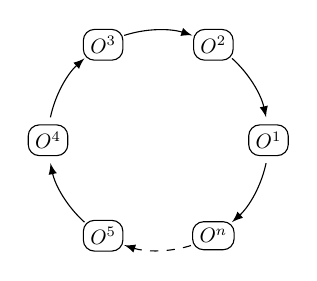
\begin{tikzpicture}[
		circle/.style={
			scale=0.75,
			rounded corners,
			draw=black, 
			text centered,
		}
		]
		
		\def \n {6}
		\def \m {4}
		\def \radius {1.4cm}
		\def \margin {12} 
		
		\foreach \s in {1,...,\m}
		{
			\node[draw, circle] at ({360/\n * (\s - 1)}:\radius) {$O^\s$};
			\draw[<-, >=latex] ({360/\n * (\s - 1)+\margin}:\radius) 
			arc ({360/\n * (\s - 1)+\margin}:{360/\n * (\s)-\margin}:\radius);
		}
		
		\node[draw, circle] at ({360/\n * 4}:\radius) {$O^5$};
		\draw[<-, dashed, >=latex] ({360/\n * 4+\margin}:\radius) 
		arc ({360/\n * 4+\margin}:{360/\n * (5)-\margin}:\radius);
		
		\node[draw, circle] at ({360/\n * 5}:\radius) {$O^n$};
		\draw[<-, >=latex] ({360/\n * 5+\margin}:\radius) 
		arc ({360/\n * 5+\margin}:{360/\n * (6)-\margin}:\radius);
		
		
		\end{tikzpicture}
		
	\caption{링 합의}
	\label{fig:settlement}
	\end{figurehere}
\end{center}

\verb|LPSC|는 거래를 진행하기 위해 \verb|TokenTransferDelegate| 스마트 계약을 사용한다. 이러한 위임자의 도입은 모든 주문이 프로토콜의 다른 버전이 아닌 해당 위임자에게 권한을 부여하기만 하면 되기 때문에 프로토콜 스마트 계약을 쉽게 업그레이드 할 수 있다.

주문링에 대한 각 주문을 위해, 실행에 따라 다음 또는 이전 주문에 대한 토큰 \verb|TokenS|의 지불이 이뤄진다. 그런 다음, 링 채굴자가 선택한 비용 모델에 따라 링 채굴자 비용이 지불된다. 마지막으로, 모든 거래가 이뤄지면, \verb|RingMined|(채굴된링) 이벤트가 내보내진다.

\subsubsection{이벤트 발생\label{sec:events}}

이 프로토콜은 릴레이, 주문 브라우저 및 기타 행위자들이 주문서 업데이트를 가능한 한 효율적으로 받을 수 있도록 해주는 이벤트를 내보낸다. 발생 이벤트는 다음과 같다:

\begin{itemize}
	\item \textbf{주문 취소(OrderCancelled)}: 특정 주문이 취소되었다.
	\item \textbf{주문들 취소(OrdersCancelled)}: 소유한 주소로부터 진행된 거래 페어의 모든 주문이 취소되었다.
	\item \textbf{모든 주문 취소(AllOrdersCancelled)}: 소유한 주소로부터 진행된 모든 거래 페어의 모든 주문이 취소되었다.
	\item \textbf{채굴된 링(RingMined)}: 주문링이 성공적으로 자리를 잡았다. 본 이벤트는 각 내부 링 토큰 전송과 관련된 데이터를 포함한다.
\end{itemize}



\section{LRx 토큰\label{sec:token}}

LRx는 우리의 일반적인 토큰 표기법이다. LRC는 이더리움 (Ethereum) 위의 루프링 토큰이고, Qtum위의 LRQ, NEO위의 LRN 등이다. 루프링이 다른 공공 블록 체인에 배치되므로, 기타 LRx 유형은 나중에 소개될 것이다.

\subsection{비용 모델\label{sec:fee_model}}
사용자가 주문을 할 때, 그들은 링 채굴자가 주장할 수 있는 주문으로부터 생성된 마진의 백분율 \verb|(marginSplitPercentage)|과 함께, 링 채굴자에게 지불될 비용으로 LRx의 금액을 지정한다. 이것을 마진분할이라고 한다. 어떤 것을 선택할 것인가의 결정은(비용 또는 마진 분할) 링 채굴자에게 달려 있다. 

마진 분할 묘사:

\begin{center}
	\begin{figurehere}
		\centering
		\begin{tikzpicture}[
		scale=1,
		font=\bfseries\footnotesize\sffamily,
		classical/.style={thick,<->,shorten >=2pt,shorten <=2pt,>=stealth},
		oneway/.style={->,dashed,shorten >=2pt,shorten <=2pt,>=stealth}
		]
		% Draw axes
		\draw [->,thick] (0,1) node (yaxis) [above] {$$}
		|- (6.2,0) node (xaxis) [right] {$$};
		
		\draw
		(4,0) coordinate (A)
		(4,1) coordinate (A2)
		(4.8,-0.6) coordinate (B)
		(4.8,1) coordinate (B2)
		(6,-0.6) coordinate (C)
		(6,1) coordinate (C2);
		
		\fill [draw=none, fill=gray!20] 
		(4.8, 0) rectangle (6, 1);
		
		\fill [draw=none, fill=gray!10] 
		(0, -0.6) rectangle (4.8, 0);
		\draw[thick] (0, -0.6) -- (0, 0.6) node[below]{$$};
		\draw[thick, thin] (A) -- (A2) node[below]{$$};
		\draw[thick, thin] (B) -- (B2) node[below]{$$};
		\draw[thick] (C) node[below, xshift=0.5cm]{총구매량} -- (C2) ;
		
		\draw[classical] (0, 0.5) -> (4, 0.5) node[below]{$$};
		\draw[classical] (4, 0.75) -> (4.8, 0.75) node[below]{$$};
		\draw[classical] (4, 0.25) -> (6, 0.25) node[below]{$$};
		
		\draw[oneway] (2, 1.2) node[above]{초기주문구매량} -- (2, 0.5);
		\draw[oneway] (4.4, 2.2) node[above]{추가구매량} -- (4.4, 0.75);
		\draw[oneway] (5.4, 1.6) node[above]{마진분할} -- (5.4, 1);
		\draw[oneway] (5, -1.2) node[below]{마진} -- (5, 0.25);
		\draw[oneway] (2.4, -1.2) node[below]{주문실제구매량} -- (2.4, -0.5);
		\end{tikzpicture}
		
	\caption{A 60\%의 마진 분할}
		\label{fig:marginsplit}
	\end{figurehere}
\end{center}

주문링의 마진이 너무 적을 경우, 링 채굴자는 LRx비용을 선택할 것이다. 반면, 결과적 마진 분할이 LRx 비용보다 훨씬 더 가치 있어 지도록 조합할 수 있는 거래가 있는 경우, 링 채굴자는 마진 분할을 선택할 것이다. 하지만, 또 다른 조건이 있다: 링 채굴자가 마진 분할을 선택할 때, 사용자(주문 작성자)에게 반드시 비용을 지불해야 하는데, 이 비용은 사용자가 링 채굴자에게 비용으로 지불했어야 할 수도 있는 LRx와 동일하다. 이로써 링 채굴자의 입장에서 주문시 부담하는 LRx 비용은 두배로 마진 분할을 택하는 경우의 한계비용이 증가하고, 이에 따라 LRx 비용을 선택하는 경향도 증가한다. 이것은 더 높은 마진의 주문링에서 더 적은 수익을 받는 것을 피하기 위해 링 채굴자가 일정한 수입을 받는 것을 선택하도록 한다. 우리의 비용 모델은 시장이 성장하고 성숙해진 만큼의 기대를 바탕으로 하고 있으며, 높은 마진 주문링이 적어질 것이다. 따라서 고정 LRx 비용이 인센티브로써 필요하게 된다.

우리는 다음과 같은 그래프를 만들게 되었다:

\begin{center}
	\begin{figurehere}
		\centering
		\begin{tikzpicture}[
		font=\bfseries\footnotesize\sffamily,
		oneway/.style={->,dashed,shorten >=2pt,shorten <=2pt,>=stealth},
		scale=1]
		% Draw axes
		\draw [<->,thick] (0,2.7) node (yaxis) [above] {$y$}
		|- (5,0) node (xaxis) [right] {$x$};
		
		\draw
		(1,1) coordinate (A)
		(2,1) coordinate (B);
		
		
		\draw[thick] (B) -- (3.7,2.7);
		\draw[dotted] (B) -- (2,0) node[below] {$2f$};
		\draw[dotted] (A) -- (1,0) node[below] {$f$};
		\draw[thick,color=gray!70] (0,0) -- (2.7,2.7);
		\draw[thick] (0,1) node[left] {$f$}--(B) node[     ]{$$};
		\draw[oneway] (4,1) node[right]{채굴 기대 수익} -- (3, 2);
		
		
\end{tikzpicture}
\caption{루프링 비용 모델}
\label{fig:feemodel}
\end{figurehere}
\end{center}
		
$f$는 LRx 비용이고, $x$는 마진 분할, $y$는 채굴 수익이다. 굵은 선으로 나태낸 것이 $y=max(f, x-f)$이다. 만약 주문을 위한 LRx 비용이 $0$이라면, 방정식은 $y=max(0, x - 0)$이고, 회색선으로 표시된 $y = x$로 단순화한다.

그 결과는:

\begin{enumerate}
      \item 마진 분할이 0이면, 링 채굴자는 낮은 LRx 비용을 선택할 것이며, 여전히 인센티브를 받게 된다.
      \item LRX 비용이 0이면, 회색 선이 나오며, 수익은 일반 직선형의 모델에 기초하여 계산된다.
      \item 마진 분할 소득이 (LRx 비용의)2배 이상일 경우, 링 채굴자는 마진 분할을 선택하고 사용자에게 LRx를 지불한다.
\end{enumerate}

LRx 비용이 0이 아니라면, 링 채굴자가 선택하는 옵션에 관계 없이, 항상 링 채굴자와 주문 발송자 사이에 LRx의 전송이 발생된다는 점에 유의해야 한다. 링 채굴자가 LRx 비용을 얻거나, 마진 분할을 받기 위해 발송인에게 LRx 비용을 지불해야한다. 

링 채굴자는 일정 비율의 비용을 월렛과 공유할 것이다. 사용자가 월렛을 통해 주문을 하고 조건이 충족되어지면, 해당 월렛은 비용 혹은 마진 분할의 일부를 보상 받게 된다. 물론 이것은 모듈단위로 이뤄지고, 이를 통한 독특한 비즈니스 모델 혹은 시행이 가능하긴 하지만, 우리는 월렛이 비용의 약 20\%-25\%를 받게 되는 것을 의도하고 있다. 월렛은 사용자 기반을 가지고 있으나 소득이 거의 없거나 아예 없기 때문에 루프링 프로토콜으로의 통합의 주 타겟으로 삼는다.

\subsection{탈중앙화 관리}

루프링 프로토콜은 효과적으로 맴버들이 목표를 달성하기 위한 운영방식의 설정을 맴버들간의 조정에 의존한다는 점에서 사회적 프로토콜이다. 이것은 일반적인 암호 경제 프로토콜과 다르지 않으며, 실제로 그것의 유용성은 주로 동일한 조정 문제 메커니즘 \cite{vitalikgovernance}, 그림 트리거(grim trigger) 상태, 그리고 제한된 합리성에 의해 보호된다. 이를 위해, LRx 토큰은 비용을 지불하는 데 사용될 뿐만 아니라 다양한 네트워크 참여자들의 재정적 인센티브를 조정하는 데도 사용된다. 이러한 조정은 프로토콜의 광범위한 채택을 위해서도 필요하지만, 성공이 주로 튼실한 분산형 생태계의 유동성 개선에 달려 있다는 점을 고려할 때, 특히 거래 프로토콜을 위해서 필요하다.

LRx 토큰은 분산된 관리를 통해 프로토콜의 갱신을 달성하는 데 사용될 것이다. 스마트 계약 업데이트는 부분적으로 연속성과 안전성을 보장하고, 비호환성을 통해 빨아들인 유동성의 리스크를 희석하기 위해 토큰 소유자에 의해 관리되어질 것이다. 스마트 계약은 한번 구축된 이후에는 변경할 수 없으며, dApps나 최종 사용자가 더 이상 사용되지 않는 버전과 계속 상호 작용하여 그들이 최신의 계약을 못하게 되는 위험이 있다. 업그레이드 능력은 시장 수요를 충족시키고 하부 블록체인들의 요구를 충족시켜야 하기 때문에 프로토콜의 성공에 핵심적인 영향을 미친다.
LRx 주주에 의한 분산된 관리 방식은 dApps 혹은 최종 사용자를 방해하지 않거나 스마트 계약 개념에 지나치게 의존하지 않고도 프로토콜 스마트 계약 업데이트를 수행할 수 있도록 할 것이다. LRx 토큰에는 고정된 공급 장치가 있으며, LRC의 경우, 전체 코인의 일부분이 루프링 재단에 동결되어 있고, 지역 사회 목적의 펀드로 할당되어 있다 \cite{LRCtokendoc}.

하지만, LRx 토큰 소유주들은 프로토콜의 방향을 조종하는 데 있어 고려해야 할 유일한 이해 당사자가 아니다: 즉, 릴레이/링 채굴자, 월렛, 개발자, 그 외 등은 생태계의 필수적인 부분이며 그들의 주장은 반드시 전해져야 한다.  실제로 이러한 에이전트는 그들 각자의 역할을 수행하기 위해 LRx를 가지고 있을 필요가 없기 때문에(기존 제조자/수신자 및 시장 형성자가 존재하지 않으므로 최초 토큰 소유는 필수가 아니다), 우리는 반드시 그들의 이율이 보장될 수 있는 대안을 인정해야한다. 또한, 투표자의 낮은 투표율과 소유권이 집중될 수 있다는 위험을 내포하고 있기 때문에, 단순한 토큰의 수에 기반 한 투표는 온/오프 체인 모두의 합의를 이끌어낼 수 없는 불완전한 방법이다.  따라서, 달성해야 할 목표는 레이어들이 내장되어 있고 일부 의사 결정 프로세스들의 세트가 표준이라는 공유된 지식에 기초하는 지배 관리 모델을 구현하는 것이다.  이것은 다양한 참가자 집합, 또는 사전에 설립된 프로토콜의 중앙에서 각종 신호를 제공하는 조정 기관에 의해 가능할 수 있다. 이것이 결실을 맺게 되면, 루프링 재단은 프로토콜 개발자에서 프로토콜 관리자로 진화할 것이다.



\section{사기와 공격으로부터의 보호}

\subsection{전면 실행 보호\label{sec:dual_authoring}}
탈 중앙화 거래소에서, 전면 실행은 누군가가 다른 노드의 무역 솔루션을 복사하려고 하거나 보류 중인 거래 풀\verb|(mempool)|에 있는 최초 거래 이전에 채굴하려고 할 때 발생한다. 이는 더 높은 거래 비용(가스 가격)을 지정하여 달성될 수 있다. 루프링(주문 매칭을 위한 모든 프로토콜)에서 발생할 수 있는 전면 실행의 주요한 방법은 주문 절도(order-filch)다: 전면 실행자가 대기 중인 주문링 합의 거래로부터 한개 이상의 주문을 훔치는 것; 그리고 루프링만의 특수한 경우로는: 전면 실행자가 대기 중인 거래로부터 주문링 전체를 훔쳤을 때가 있다.

링제출\verb|(submitRing)| 거래가 확인되지 않고, 여전히 거래 풀에서 보류중일 때, 누구나 해당 거래를 쉽게 발견할 수 있고 자신의 주소 \verb|(filcherAddress)|로 기존의 채굴주소\verb|(minerAddress)|를 대체할 수 있다. 그리고 나서, \verb|filcherAddress|로 바꾼 페이로드\verb|(payload)|로 주문링에 재서명할 수 있다. 플리처들은 더 높은 가격을 설정하고 블록 채굴자들이 다음 블록에 기존 링제출\verb|(submitRing)| 거래가 아닌 그들이 만든 새 거래를 선정하기를 바라며 새로운 거래를 제출할 수 있다.
이 문제에 대한 이전의 해결책은 중요한 단점을 가지고 있었다: 더 많은 거래를 요구하고 따라서 링 채굴자들은 더 많은 가스를 지출해야 한다는 것이었다. 우리의 새로운 솔루션, 이중 인증\verb|(Dual Authoring)|\cite{dualauthor}은 주문에 대해 두가지 레벨의 승인을 설정하는 메커니즘을 포함하고 있다. 하나는 정착용이고, 다른 하나는 링 채굴용이다.

이중 인증 과정:

\begin{enumerate}

      \item 각 주문에 대해, 월렛 소프트웨어는 무작위 공공 키/개인 키 페어를 생성하고, 그 키 페어를 주문의 \verb|JSON| snippet에 연결한다. (대안은 byte 사이즈를 줄이기 위해 자체 공개 키 대신 공개 키에서 파생된 주소를 사용하는 것이다. 이러한 주소를 표시하기 위해 \verb|authAddr|를 사용되고, \verb|authAddr|와 매칭되는 개인 키를 나타내기 위해 \verb|authKey|를 사용한다).
     
      \item r, v, s및 \verb|authKey|를 제외한 주문의 모든 필드에 주문 해시를 계산하고, 소유주의 개인 키(\verb|authKey|가 아님)를 사용해 해시에 서명한다. 
      
      \item 월렛은 주문서와 함께 링 채굴을 위해 \verb|authKey|와 릴레이에 보내질 것이다. 링 채굴자는 \verb|authKey|와 \verb|aauthAddr|가 정확하게 페어를 이루고 있고 주문의 서명이 소유주 주소에 대해 유효한지 인증할 것이다. 
      
      \item 주문링이 확인되면 링 채굴자는 링의 해시, 채굴자 주소\verb|(minerAddress)|, 그리고 모든 채굴 매개 변수에 서명하기 위해 각 주문의 \verb|authKey|를 사용할 것이다. 주문링에 n개의 주문이 포함된 경우, n개의 \verb|autheKys|에 의해 n개의 서명이 있을 것이다. 우리는 이러한 서명을 \verb|authSignature|s라 부른다. 또한, 링 채굴자는 모든 채굴 매개 변수를 갖춘 링 해시와 함께 서명해야 할 필요도 있다. 
      
      \item 링 채굴자는 모든 매개 변수와 함께 링제출 \verb|(submitRing)| 기능과 추가적인 \verb|authSignature|s 기능도 호출한다. \verb|authKey|는 온체인 거래의 부분이 아니고, 따라서 링 채굴자 외 다른 외부인에게는 알려지지 않은 채로 남아 있다는 것을 알린다.
     
      \item 이제 루프링 프로토콜은 각 주문의 해당 \verb|authAddr|에 반하는 각 \verb|authSignature|를 인증할 것이며, \verb|authSignature|가 없거나 유효하지 않은 경우 주문링을 거부할 것이다. 
      
\end{enumerate}

결과는 이제 다음과 같다:

\begin{itemize}

      \item  주문의 서명(소유자 주소의 개인키에 의한)은 주문이 \verb|authAddr|를 포함하여 수정될 수 없도록 보장한다. 
      
      \item  만약 제공된다면, 링 채굴자의 서명(채굴자 주소의 개인키에 의한)은 그 누구도 주문링을 채굴하기 위해 그의 신분을 사용할 수 없도록 보장한다.
      
      \item \verb|authSignature|s은 \verb|minerAddress|(채굴자 주소)를 포함해, 전체 주문링이 수정될 수 없고, 어떤 주문도 도난당하지 않도록 보장한다. 
\end{itemize}

이중 인증(Dual Authoring)은 주문링이 여전히 한번의 거래로 행해질 수 있도록 하면서, 링 절도(ring-filch)와 주문 절도(order-filch)를 방지할 수 있다. 또한 이중 인증(Dual Authoring)은 릴레이가 매치가 불가능한 공유와 매치가 가능한 공유의 두가지 방법으로 주문을 공유 할 수 있도록 해준다.  
기본적으로, 루프링은 OTC모델을 작동하고 지정 가격 주문만 지원하도록 하는데, 주문의 타임 스탬프가 무시될 수 있음을 의미한다. 이는 전면 실행 거래가 해당 거래의 실제 가격에 영향을 미치지 않지만, 실행 여부에는 영향을 미친다는 것을 보여준다.



\section{기타공격}

\subsection{시빌(Sybil) 또는 도스(DOS) 공격}
악성 사용자들 – 그들 스스로의 모습 또는 위조된 ID로 활동하는 - 은 루프링 노드를 공격하기 위해 대량의 작은 주문들을 전송할 수 있었다. 그러나 우리는 노드가 자체 기준에 따라 - 숨기거나 드러낼 수 있는 - 주문을 거부할 수 있도록 만들었기 때문에 이러한 주문의 대부분은 매치가 되었을 때 만족스러운 이익을 내지 못하여 거부될 것이다. 릴레이가 어떻게 그들이 주문들을 관리하는지 지시할 수 있는 권한을 부여함으로써, 우리는 대량의 소규모 주문 공격을 위협으로 보지 않는다.

\subsection{불충분한 잔고}
악성 사용자는 주문 값에는 0이 아니지만 실제로는 잔고가 없는 주소를 가진 주문에 서명하고 이를 전달할 수 있었다. 노드는 일부 주문의 실제 잔액이 0이라는 것을 발견하고 모니터링하여, 이에 맞게 주문 상태를 업데이트한 다음 삭제할 수 있다. 노드는 주문 상태를 업데이트하는 데 시간을 소비해야 하지만, 예를 들어 주소 블랙 리스트 지정 및 관련 주문 삭제 등을 통해 작업량을 최소화하도록 할수도 있다.



\section{요약}
루프링 프로토콜은 탈중앙화 거래의 기초 레이어로 규정된다. 그렇게 함으로써, 프로토콜은 사람들이 자산과 가치를 어떻게 거래하는지에 대해 큰 영향을 미친다. 중간 상품으로써, 돈은 물물 교환을 용이하게 하거나 대체하고, 두 당사자가 각각의 특정한 물건과 서비스를 반드시 원해야만 거래가 이뤄질 수 있다는 욕망의 상호 일치문제(double coincidence of wants problem) \cite{unenumerated2006}의 발생을 해결한다. 마찬가지로, 루프링 프로토콜은 더 쉽게 거래를 성사시키기 위해 매칭되는 링들을 활용하여, 토큰 거래 페어에서 욕망의 상호일치 문제를 해결하는 것을 목표로 한다. 이것은 사회와 시장이 어떻게 토큰, 기존의 자산, 그리고 그 이상을 교환하는지와 관련해 의미가 있다. 실제로, 탈중앙화 암호 화폐가 한 국가의 돈에 대한 통제에 위협을 가하는 것처럼, 거래자들(소비자/생산자)을 매칭시켜주는 프로토콜은 돈 자체의 개념에 대한 이론상의 위협이 될수 있다.

루프링 프로토콜의 이점은 다음과 같다.

\begin{itemize}
      \item 오프 체인 주문 관리 및 온 체인 합의를 통해 보안성을 희생하지 않는다.
      \item 링 채굴 및 주문 공유를 통해 거대한 유동성을 확보할 수 있다.
      \item 이중 인증은 오늘날 모든 DEXs와 그 사용자들이 직면한 전면 실행의 치명적인 문제점들을 해결한다.
      \item 무료 및 공공 스마트 계약은 모든 dApp이 프로토콜을 구축하거나 프로토콜과 상호 작용할 수 있게 한다.
      \item 운영자들 간의 표준화는 네트워크 효과와 향상된 최종 사용자 경험을 가능하게 한다.
      \item 네트워크는 주문서를 운영하고 의사 소통을 하는 데 있어 유연성을 유지한다.
      \item 진입 장벽이 감소하면 네트워크 및 최종 사용자가 참여하는 노드의 비용이 절감된다.
      \item 사용자 월렛으로부터 직접 익명으로 거래하는 것이 가능하다.
      
\end{itemize}



\section{감사의 말}
우리는 우리의 멘토들, 조언자들 그리고 우리를 매우 환영해주고 그들의 지식을 공유하는데 관대했던 커뮤니티의 많은 사람들에게 감사를 표하고 싶다. 특히, Shuo Bai (ChinaLedger), Haibin Kan 교수; Alex Cheng, Hongfei Da; Yin Cao; Xiaochuan Wu; Zhen Wang, Wei Yu, Nian Duan, Jun Xiao, Jiang Qian, Jiangxu Xiang, Yipeng Guo, Dahai Li, Kelvin Long, Huaxia Xia, Jun Ma, 그리고 Encephalo Path에게 이 프로젝트를 검토하고 의견을 제공해 주셔서 감사하다고 전하고 싶다.


\bibliography{whitepaper}
\bibliographystyle{unsrt}


\end{multicols}

%

%\begin{appendices}

%

%\section{Loopring Implemented on EVM\label{app:protocol_ethereum}}

%

%\begin{center}

%\begin{figurehere}

%\centering

%\begin{tikzpicture}

%[node distance = 1cm, auto,font=\footnotesize,

%% STYLES

%every node/.style={node distance=3cm},

%% The comment style is used to describe the characteristics of each force

%comment/.style={rectangle, inner sep= 5pt, text width=4cm, node distance=0.25cm, font=\scriptsize\sffamily},

%% The force style is used to draw the forces' name

%force/.style={rectangle, draw, fill=black!10, inner sep=5pt, text width=4cm, text badly centered, minimum height=1.2cm, font=\bfseries\footnotesize\sffamily}] 

%

%% Draw forces

%\node [force] (impl) {LoopringProtocolImpl};

%\node [force, dashed, above of=impl] (protocol_interface) {LoopringProtocol};

%\node [force, left=1cm of impl] (nameregistry) {NameRegistry};

%\node [force, right=1cm of impl] (tokenregistry) {TokenRegistry};

%\node [force, below of=impl] (delegate) {TokenTransferDelegate};

%\node [force, left=1cm of delegate] (multisig) {TransferableMultsig};

%

%%%%%%%%%%%%%%%%

%% Change data from here

%

%% impl

%\node [comment, below=0.25 of impl] (comment-impl) {- Validates order-rings\\

%- Transfers tokens for settlement\\

%- Emits events};

%

%% nameregistry

%\node [comment, below=0.25cm of nameregistry]{- Registers wallets and relays};

%

%% protocol_interface

%\node [comment, below=0.25 of protocol_interface](comment-interface) {- Defines interfaces and events};

%

%% tokenregistry

%\node [comment, below=0.25 of tokenregistry] {- Registers ERC20/ERC223 tokens};

%

%% delegate

%\node [comment, below=0.25 of delegate] {- Transfers tokens on behalf of users};

%

%% PUBLIC POLICIES

%\node [comment, text width=3cm, below=0.25 of multisig] {- Enables multisignature ownership};

%

%%%%%%%%%%%%%%%%%

%

%% Draw the links between forces

%\path[->,thick] 

%(comment-interface) edge (impl)

%(nameregistry) edge (impl)

%(tokenregistry) edge (impl)

%(delegate) edge (comment-impl);

%

%\end{tikzpicture} 

%\caption{Smart Contracts}

%\label{fig:smartcontracts}

%\end{figurehere}

%\end{center}

%

%\section{Deployment}

%

%

%\subsection{Ethereum}

%The following smart contracts have been deployed on Ethereum mainnet:

%\begin{itemize}

%\item LRC: \verb|0xEF68e7C694F40c8202821eDF525dE3782458639f|

%\item TokenRegistry: \verb|0xa21c1f2AE7f721aE77b1204A4f0811c642638da9|

%\item TokenTransferDelegate: \verb|0x7b126ab811f278f288bf1d62d47334351dA20d1d|

%\item NameRegistry: \verb|0xd181c1808e3f010F0F0aABc6Fe1bcE2025DB7Bb7|

%\item LoopringProtocolImpl: \verb|0x0B48b747436f10c846696e889e66425e05CD740f|

%\end{itemize}

%

%\subsection{Qtum}

%The following smart contracts have been deployed on Qtum mainnet:

%\begin{itemize}

%\item LRQ: \verb| 2eb2a66afd4e465fb06d8b71f30fb1b93e18788d |

%\item TokenRegistry: \verb| c89ea34360258917daf3655f8bec5550923509b3 |

%\item TokenTransferDelegate: \verb| 60b3fa7f461664e4dafb621a36ac2722cc680f10 |

%\item NameRegistry: \verb| e26a27d92181069b25bc7283e03722f6ce7678bb |

%\item LoopringProtocolImpl: \verb| 5180bb56b696d16635abd8dc235e0ee432abf25d |

%\end{itemize}

%

%\end{appendices}

\end{document}